% !TeX spellcheck = pt_PT
%
%
% Capitulo 5
%
\chapter{Testes} \label{testes}
Este capítulo aborda os testes executados no projeto.

\section{Aplicação Servidor} \label{sec51}
Nesta fase do projeto, os testes feitos à partição da aplicação servidor foram executados sem a participação da aplicação cliente.

Para a execução destes testes, foram usadas duas ferramentas distintas:\\
\\
\begin{tabular}{ll}
	\emph{XAMMP} & \emph{free open-source cross-platform web server solution stack} para criar um servidor\\
	 de testes.\\
	 \\
	\emph{Postman} & API cliente para gerar pedidos HTTP.\\
	\\
\end{tabular}

No ficheiro \emph{apliccation.properties} existente na \emph{framework Spring} foram escritas as propriedades essenciais para garantir a ligação entre a aplicação e o servidor \emph{XAMMP}.

\begin{verbatim}
spring.jpa.hibernate.ddl-auto=update
spring.datasource.url=jdbc:mysql://${MYSQL_HOST:localhost}:3306/test
spring.datasource.username=root
spring.datasource.password=
\end{verbatim}

\begin{figure}[h]
	\begin{center}
		\resizebox{100mm}{!}{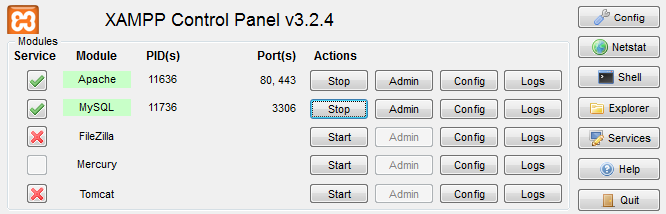
\includegraphics{./figures/xammp.png}}
	\end{center}
	\caption{Figura do painel de controlo do \emph{XAMMP}.}\label{fig:logotipo}
\end{figure}

As seguintes sub-secções demonstram os vários testes aos \emph{endpoints} da classe {\bf Evento}.\\


\subsection{Testes de GET}\label{511}
Os testes feitos aos \emph{endpoints} de \emph{GET} foram repetidos ao longo dos testes dos outros métodos para fins de observação de resultados, pelo que nesta sub-secção apenas se observam dois testes realizados antes da geração de informação de teste.\\


\begin{tabular}{ll}
	Teste : & \emph{GET ALL}\\
	\\
	\emph{Endpoint} : & http://localhost:8080/event/all\\
	\\
	\emph{Body} : & Nenhum\\
	\\
	Resultado : & Lista de objetos \emph{JSON} de todos os Eventos.\\
	\\
	\emph{Status} : & \emph{200 OK}\\
	\\
	Nota : & Para efeitos de teste, foi colocado previamente um Evento para observação.\\
\end{tabular}

\begin{figure}[h]
	\begin{center}
		\resizebox{150mm}{!}{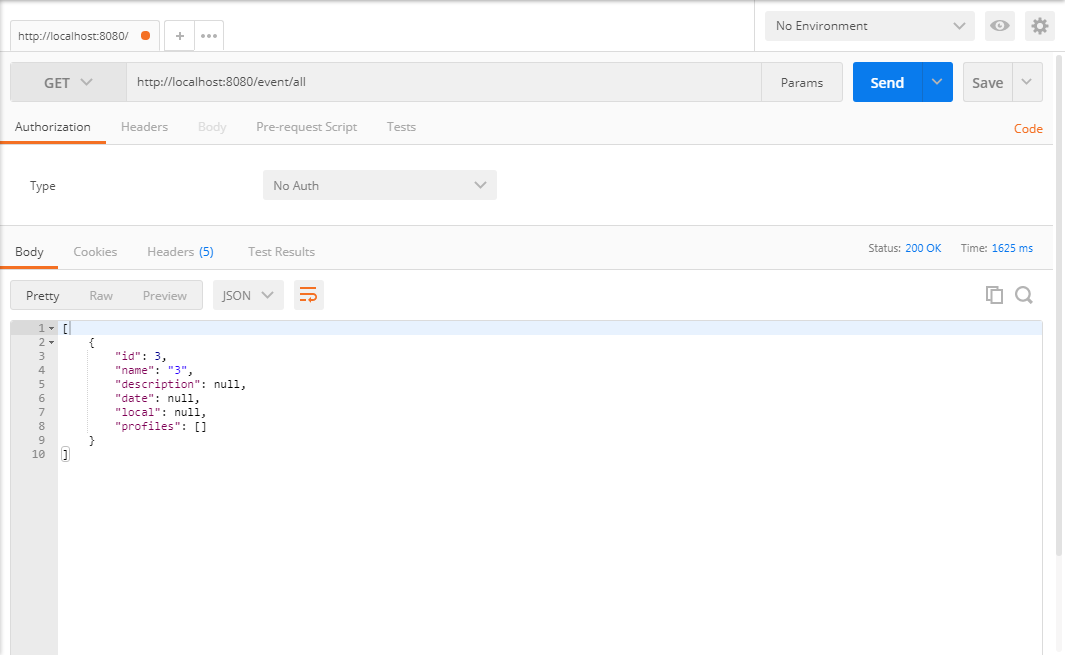
\includegraphics{./figures/eventall.png}}
	\end{center}
	\caption{Resultado observável no \emph{Postman}.}\label{fig:eventall}
\end{figure}
\newpage
\begin{tabular}{ll}
	Teste : & \emph{GET BY EXISTENT ID }\\
	\\
	\emph{Endpoint} : & http://localhost:8080/event/findById/3\\
	\\
	\emph{Body} : & Nenhum\\
	\\
	Resultado : & Objeto \emph{JSON} do evento com id 3.\\
	\\
	\emph{Status} : & \emph{200 OK}\\
	\\
	Nota : & Para efeitos de teste, foi colocado previamente um Evento com id 3 para observação. \\
\end{tabular}

\begin{figure}[h]
	\begin{center}
		\resizebox{150mm}{!}{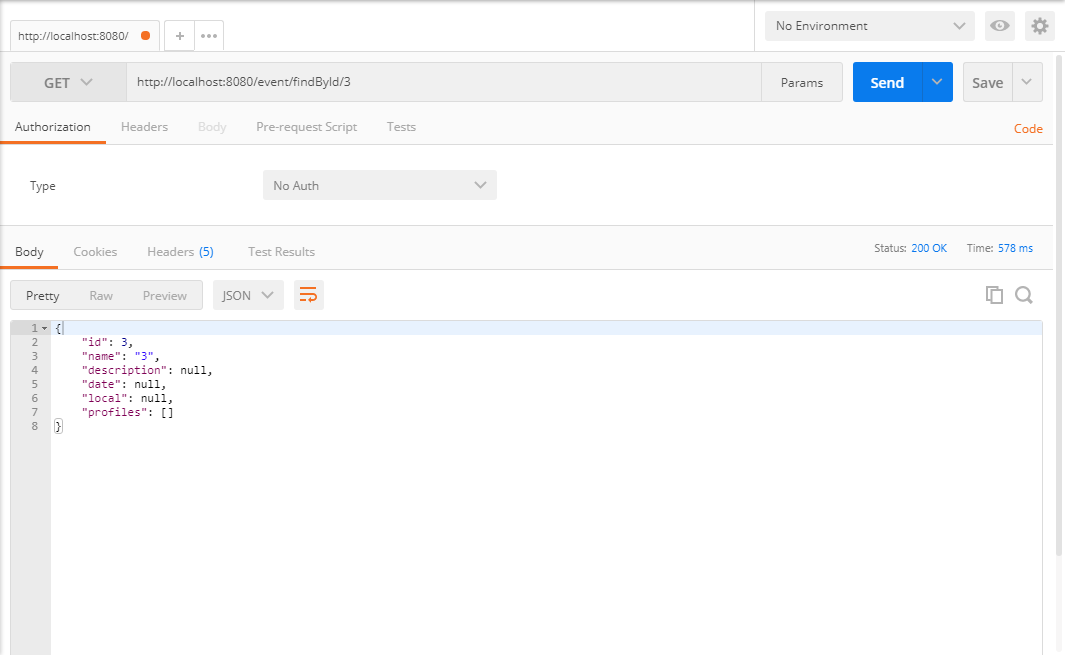
\includegraphics{./figures/eventfindbyid200.png}}
	\end{center}
	\caption{Resultado observável no \emph{Postman}.}\label{fig:eventfindbyid200}
\end{figure}
\newpage


\begin{tabular}{ll}
	Teste : & \emph{GET BY NONEXISTENT ID}\\
	\\
	\emph{Endpoint} : & http://localhost:8080/event/findById/4\\
	\\
	\emph{Body} : & Nenhum\\
	\\
	Resultado : & Erro\\
	\\
	\emph{Status} : & \emph{404 NOT FOUND}\\
	\\
	Nota : & Para efeitos de teste, foi escolhido um id que não existe na base de dados.\\
\end{tabular}

\begin{figure}[h]
	\begin{center}
		\resizebox{150mm}{!}{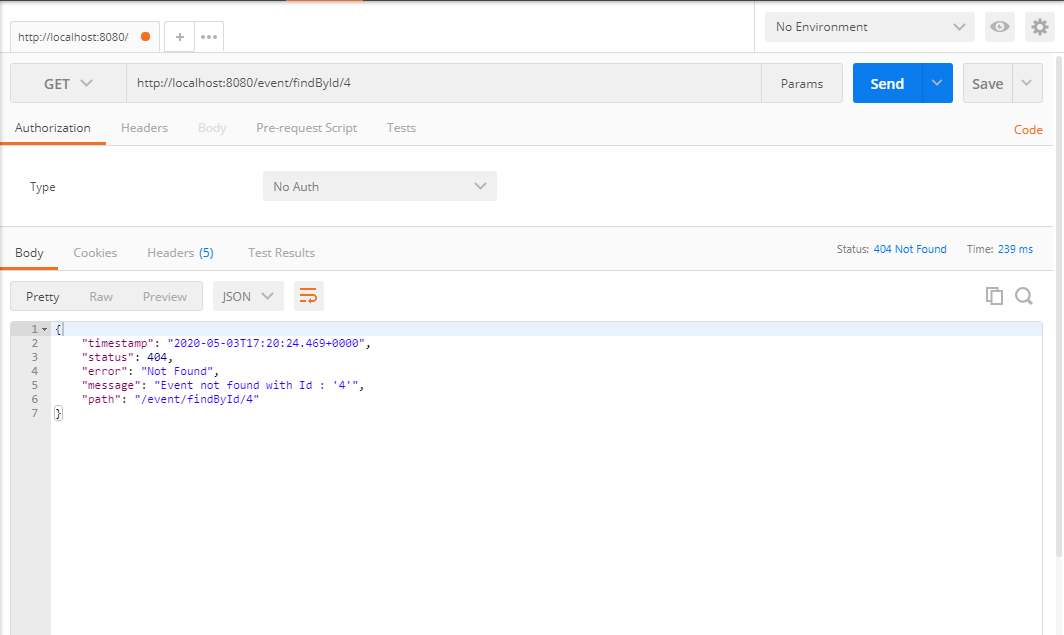
\includegraphics{./figures/eventfindbyid404.png}}
	\end{center}
	\caption{Resultado observável no \emph{Postman}.}\label{fig:eventfindbyid404}
\end{figure}
\newpage

\subsection{Testes de POST}\label{512}
Os testes feitos ao \emph{endpoint} de \emph{POST} são executados com um objecto \emph{JSON} enviado no corpo do pedido. O id não é enviado juntamente com o resto da informação do objeto, pois é um campo gerado automaticamente e é retornado no corpo da resposta.\\
\\
\begin{tabular}{ll}
	Teste : & \emph{POST}\\
	\\
	\emph{Endpoint} : & http://localhost:8080/event/post\\
	\\
	\emph{Body} : & \{ \\
				  &	"name": "TestEvent",\\
				  & "description": "Description Of TestEvent",\\
				  & "date": "2020-05-04T00:00:00.000Z",\\
				  & "local": "Portugal",\\
				  & "profiles": []\\
				  & \} \\
	\\
	Resultado : & id do objeto criado.\\
	\\
	\emph{Status} : & \emph{200 OK}\\
	\\
\end{tabular}

\begin{figure}[h]
	\begin{center}
		\resizebox{150mm}{!}{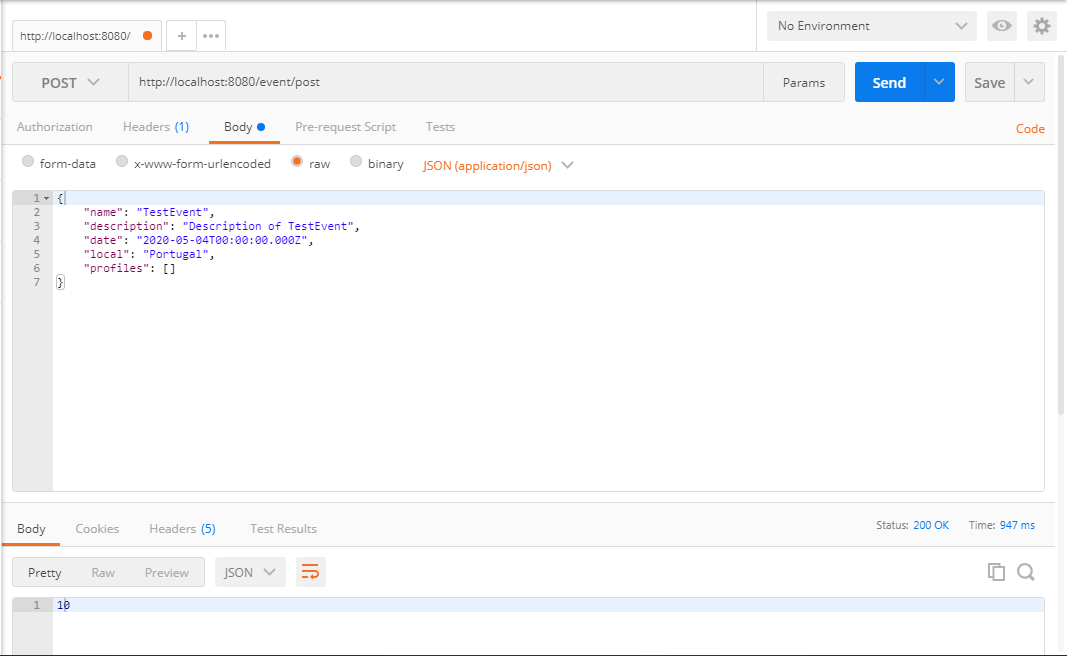
\includegraphics{./figures/eventpost.png}}
	\end{center}
	\caption{Resultado observável no \emph{Postman}.}\label{fig:eventfindbyid404}
\end{figure}
\newpage
\begin{figure}[h]
	\begin{center}
		\resizebox{150mm}{!}{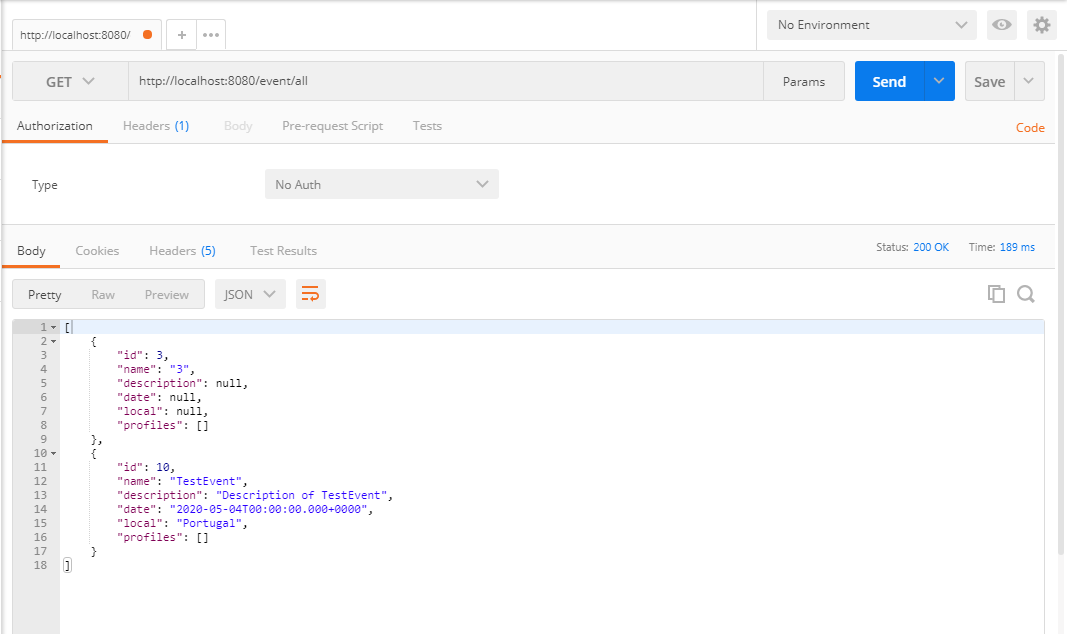
\includegraphics{./figures/eventallafterpost.png}}
	\end{center}
	\caption{Resultado de um \emph{GET ALL} depois do \emph{POST} observável no \emph{Postman}.}\label{fig:eventallafterpost}
\end{figure}
\newpage

\subsection{Testes de UPDATE}\label{513}
Os testes feitos ao \emph{endpoint} de \emph{UPDATE} são executados com um objecto \emph{JSON} enviado no corpo do pedido com o id do objeto a ser alterado, assim como os campos a alterar. O id continua a ser retornado no corpo da resposta.\\
\\
\begin{tabular}{ll}
	Teste : & \emph{UPDATE EXISTENT OBJECT}\\
	\\
	\emph{Endpoint} : & http://localhost:8080/event/update\\
	\\
	\emph{Body} : & \{ \\
	& "id": 10, \\
	& "name": "TestEventUpdated",\\
	& "description": "Updated Description Of TestEvent",\\
	& "date": "2020-05-05T00:00:00.000Z",\\
	& "local": "Spain",\\
	& "profiles": []\\
	& \} \\
	\\
	Resultado : & id do objeto alterado.\\
	\\
	\emph{Status} : & \emph{200 OK}\\
	\\
\end{tabular}

\begin{figure}[h]
	\begin{center}
		\resizebox{150mm}{!}{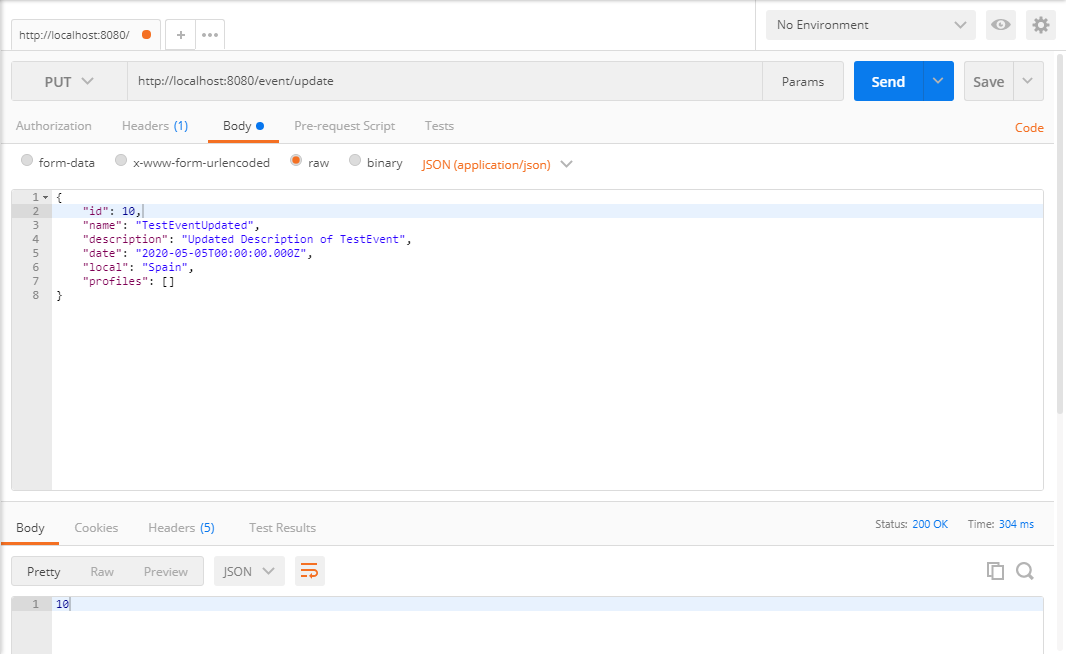
\includegraphics{./figures/eventput.png}}
	\end{center}
	\caption{Resultado observável no \emph{Postman}.}\label{fig:eventput}
\end{figure}
\newpage
\begin{figure}[h]
	\begin{center}
		\resizebox{150mm}{!}{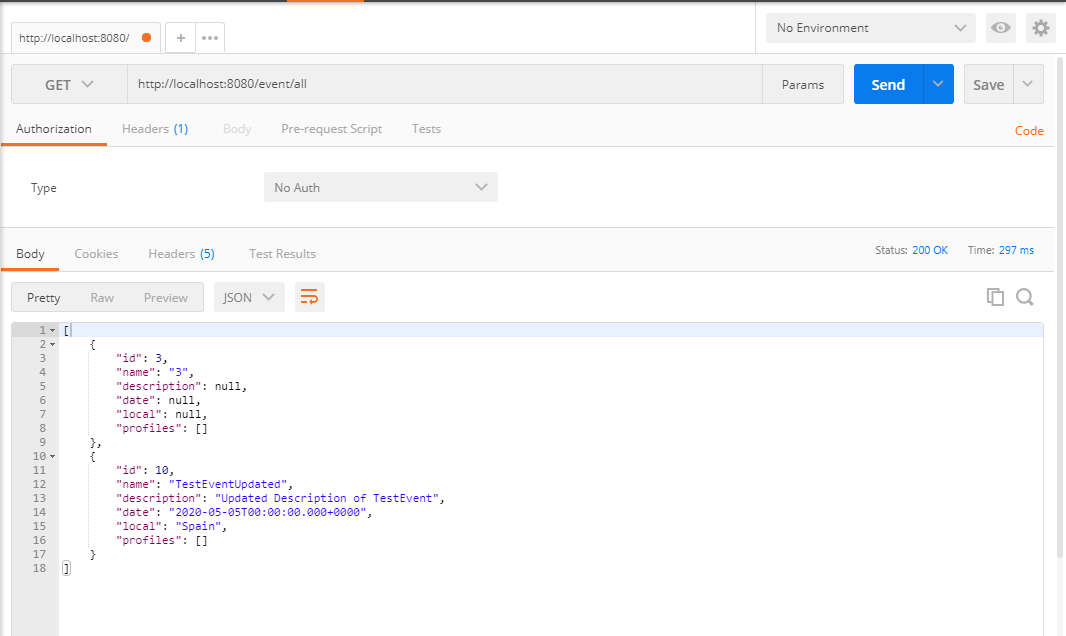
\includegraphics{./figures/eventallafterput.png}}
	\end{center}
	\caption{Resultado de um \emph{GET ALL} depois do \emph{PUT} observável no \emph{Postman}.}\label{fig:eventallafterput}
\end{figure}
\newpage

\begin{tabular}{ll}
	Teste : & \emph{UPDATE NONEXISTENT OBJECT}\\
	\\
	\emph{Endpoint} : & http://localhost:8080/event/update\\
	\\
	\emph{Body} : & \{ \\
	& "id": 9 \\
	& "name": "TestEventUpdated",\\
	& "description": "Updated Description Of TestEvent",\\
	& "date": "2020-05-05T00:00:00.000Z",\\
	& "local": "Spain",\\
	& "profiles": []\\
	& \} \\
	\\
	Resultado : & Erro.\\
	\\
	\emph{Status} : & \emph{404 NOT FOUND}\\
	\\
\end{tabular}

\begin{figure}[h]
	\begin{center}
		\resizebox{150mm}{!}{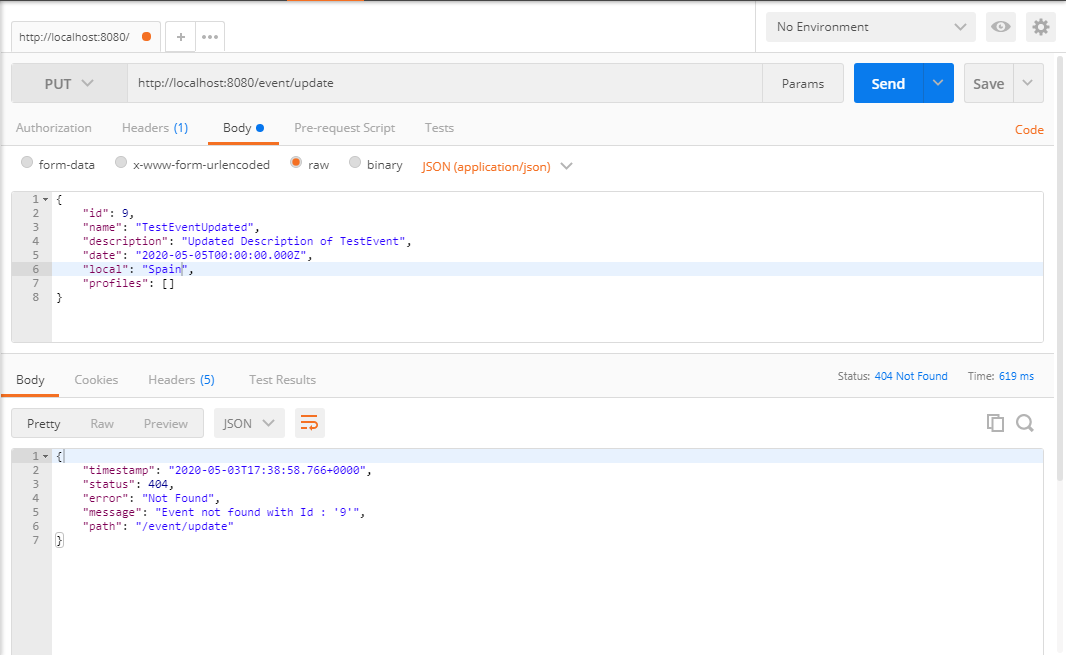
\includegraphics{./figures/eventput404.png}}
	\end{center}
	\caption{Resultado observável no \emph{Postman}.}\label{fig:eventput404}
\end{figure}
\newpage

\subsection{Testes de DELETE}\label{514}
Os testes feitos ao \emph{endpoint} de \emph{DELETE} são executados com um objecto \emph{JSON} enviado no corpo do pedido com o id do objeto a ser apagado.\\
\\
\begin{tabular}{ll}
	Teste : & \emph{DELETE EXISTENT OBJECT}\\
	\\
	\emph{Endpoint} : & http://localhost:8080/event/delete\\
	\\
	\emph{Body} : & \{ \\
	& "id": 10 \\
	& \} \\
	\\
	Resultado : & Nenhum\\
	\\
	\emph{Status} : & \emph{200 OK}\\
	\\
\end{tabular}

\begin{figure}[h]
	\begin{center}
		\resizebox{150mm}{!}{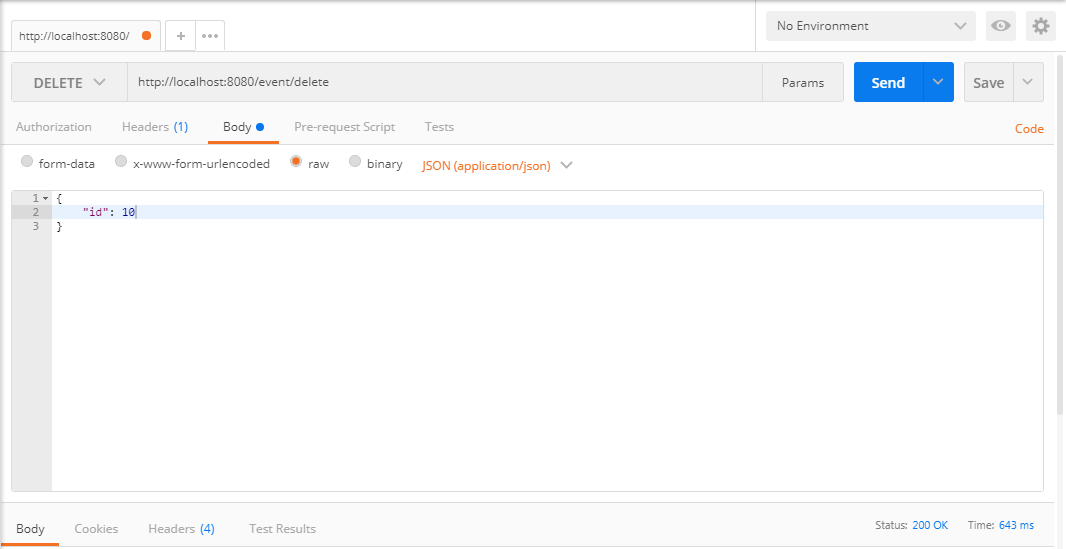
\includegraphics{./figures/eventdelete.png}}
	\end{center}
	\caption{Resultado observável no \emph{Postman}.}\label{fig:eventdelete}
\end{figure}
\newpage
\begin{figure}[h]
	\begin{center}
		\resizebox{150mm}{!}{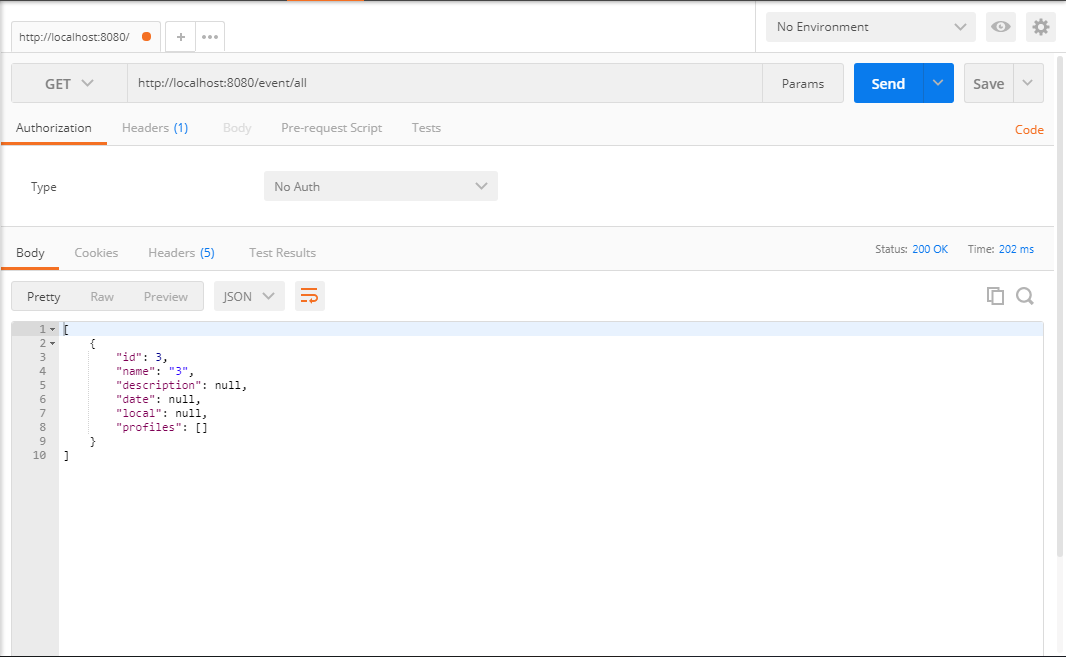
\includegraphics{./figures/eventallafterdelete.png}}
	\end{center}
	\caption{Resultado de um \emph{GET ALL} depois do \emph{DELETE} observável no \emph{Postman}.}\label{fig:eventallafterdelete}
\end{figure}
\newpage
\begin{tabular}{ll}
	Teste : & \emph{DELETE NONEXISTENT OBJECT}\\
	\\
	\emph{Endpoint} : & http://localhost:8080/event/delete\\
	\\
	\emph{Body} : & \{ \\
	& "id": 9 \\
	& \} \\
	\\
	Resultado : & Erro\\
	\\
	\emph{Status} : & \emph{404 NOT FOUND}\\
	\\
\end{tabular}

\begin{figure}[h]
	\begin{center}
		\resizebox{150mm}{!}{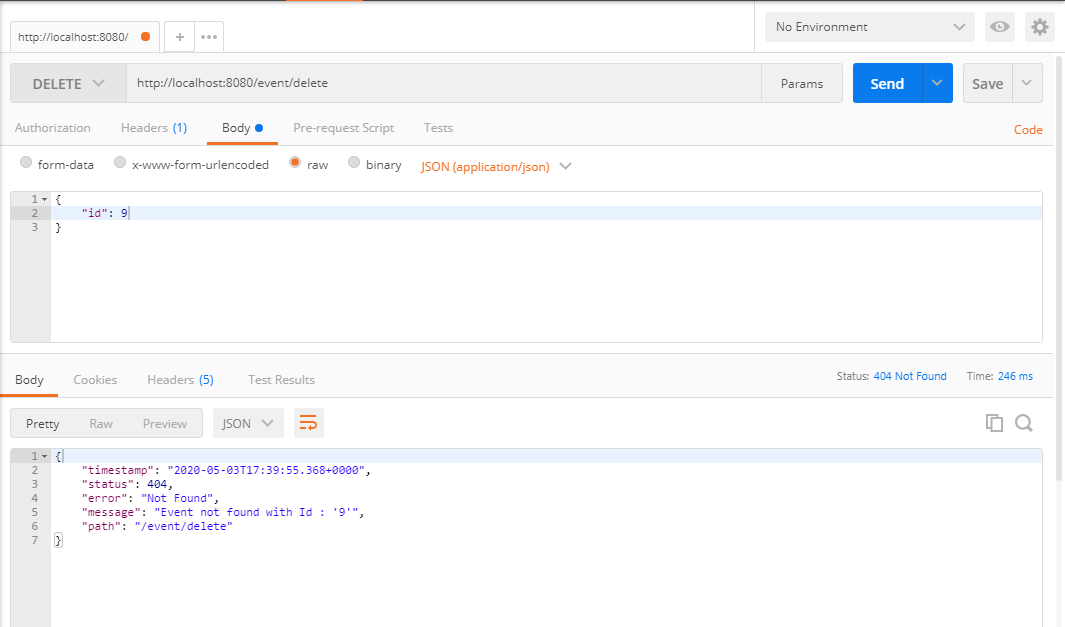
\includegraphics{./figures/eventdelete404.png}}
	\end{center}
	\caption{Resultado observável no \emph{Postman}.}\label{fig:eventdelete404}
\end{figure}